

\chapter{Molecular Vibrations}



\section{Tasks}

\begin{itemize}
\item Get  the raw data of the absorption and emission spectra of the dye BODIPY 650/665 from \href{https://www.thermofisher.com/de/de/home/life-science/cell-analysis/labeling-chemistry/fluorescence-spectraviewer.html?SID=srch-svtool&UID=10001moh}{thermofischer.com}.
 Convince yourself that the mirror-law holds.




\item Make an as accurate as possible sketch of the potentials of ground and excited state of BODIPY 650/665, assuming that only one vibrational mode contributes.

\end{itemize}


\begin{marginfigure}
   \includestandalone[width=\textwidth]{\currfiledir fig_bodipy}
  \caption{Absorption and emission spectrum of  the BODIPY dye.}
\end{marginfigure}





\section{Franck-Condon and Huang-Rhys}

A molecule with an electronic ground state $g$ and electronic excited state $e$ can undergo periodic oscillations of the nuclei positions along a coordinate $r$. We assume\footcite{Kuzmany} that the potential of these oscillations is harmonic, i.e.
\begin{eqnarray*}
 U_g(r) &=& \frac{1}{2} \, k\, r^2 = \frac{1}{2} \, m \, \omega^2 \, r^2 \\
  U_e(r) &=&  U_g(r) + E_{eg} - A \, r = E_{eg}  - A \, r + \frac{1}{2} \, m \, \omega^2 \, r^2 
 \end{eqnarray*}
where $E_{eg}$ is the electronic contribution to the energy difference. We assumed that both potentials have the same shape, i.e., the same vibrational frequency. The term $A \, r$ couples the electronic state and the nuclear oscillator. It shifts the excited state potential along the $r$ coordinate. While the ground state potential has its minimum at $r=0$, the minimum for the excited state is at
%
%
\begin{marginfigure}
   \includestandalone{\currfiledir fig_parabula}
\caption{The coupling term $-A r$ in the potential of the excited state $e$ shifts the minimum of the parabola to larger values of $r$ and lower values of the potential. }
\end{marginfigure}
%
%
\[
 A = m \, \omega^2 \,  r	 \quad \text{i.e.} \quad r = \frac{A}{m \omega^2}
\]
The energies of the quantum mechanical eigenstates are 
\begin{eqnarray*}
  E_{g, n} &=&  (n + 1/2) \, \hbar \omega  \\
  E_{e, m} &=&  (m + 1/2) \, \hbar \omega  +  E_{eg} - \frac{A^2}{2 m \omega^2} =
   (m + 1/2 - S^2) \, \hbar \omega  +  E_{eg} 
\end{eqnarray*}
We introduce the Huang-Rhys factor $S$ as dimensionless coupling constant
\[
 S = \frac{A}{\hbar \omega} \sqrt{\frac{\hbar}{2 m \omega}} \quad .
\]
The eigenfunctions $\chi_n$ of the nuclear vibrations are Hermite polynomials. The Franck-Condon factor describes the overlap integral of the vibrational wavefunction of ground and excited state. As the electronic transition is fast compared to nuclear motion, the nuclear coordinate can not change during the transition (Born-Oppenheimer approximation), and both ground and excited state need a non-vanishing probability to be at the same coordinate $r$. When one of the states is in a vibrational ground state, i.e., $n$ or $m$ equals zero, the Franck-Condon factor takes the form
\[
 | \braket{ \chi_0 | \chi_m } | ^2  =  | \braket{ \chi_m | \chi_0 } | ^2 = \frac{S^m \exp(-S)}{m!}
\]
which is a Poisson distribution of mean value $S$.  The strongest transition is thus the transition into $m \approx S$, which for large coupling between electronic and nuclear system, i.e. large $S$, will deviate from the 0--0 transition.

\begin{figure}
   \includestandalone[width=10cm]{\currfiledir fig_poisson}
  \caption{Poisson distributions}
\end{figure}

The Debye-Waller factor $D$ gives the ratio of the coherently scattered wave to all scattering processes. For molecules, this corresponds to the amplitude of the 0--0 line to the integral over the whole band. As the sum over all Franck-Condon factors to the same final state is one, we get
\[
 D =  | \braket{ \chi_0 | \chi_0 } | ^2 = \exp(-S)
\]


\section{Stokes shift and mirror rule}


When we keep the assumptions of the last section, that vibrational frequency of ground end excited state are the same, both potentials are harmonic, and of course the Born-Oppenheimer approximation hold, then absorption and emission spectrum are closely related. The 0--0 transition at energy $E_{00}$ from the vibrational ground state of the electronic ground state to the vibrational ground state of the electronic excited state appears both in absorption and emission. As the thermal energy $kT$ is in most cases small compared to the vibrational energy $\hbar \omega$, almost all molecules are in the vibrational ground state. Absorption then only occurs at energies larger than $E_{00}$ into higher vibrational state of the electronic excited state. These energies are
\[
  E_{abs, n} = E_{00} + n \, \hbar \omega
\]
Fluorescence emission also occurs out of a vibrational ground state, but due to different reasons than absorption. In molecules, vibrational relaxation  (some ps) is much faster\sidenote{'Faster' means here that the rates are larger. The event itself can be assumed to be instantaneous. } than fluorescence emission (some ns). The emission occurs thus into different vibrational levels of the electronic ground state at
\[
  E_{em, n} = E_{00} - n \, \hbar \omega
\]
The spectral position of the absorption and emission peaks are thus mirrored around the 0--0 transition  energy $E_{00}$.

Not only the spectral positions, but also the amplitude of the peaks in absorption spectrum $\epsilon(\omega)$ and fluorescence spectrum $F(\omega)$ are related. The reason is that the Einstein $A$ and $B$ coefficients are related, or that there is only one transition dipole moment $\mu$ which governs both absorption and emission. The only caveat is the relation between the transition dipole moment and the spectra\footcite[Chapter 5.2]{Parson}
\begin{eqnarray*}
   \epsilon(\omega  =  \omega_{g,m \rightarrow e,n} )  & \propto & \omega_{g,m \rightarrow e,n}  \,  | \braket{\chi_n |  \chi_m} |^2 
\, B_{eg} \\
   F(\omega =  \omega_{e,n \rightarrow g,m} ) & \propto & \omega_{e,n \rightarrow g,m}^3 \,  | \braket{\chi_m |  \chi_n} |^2 
\, B_{ge}
\end{eqnarray*}
In each case, one factor of $\omega$ appears due to the photon energy $\hbar \omega$, as the right-hand side considers single absorption or emission events,  but the right-hand side uses spectra in terms of power per spectral interval, not photons. The fluorescence spectra gets an additional factor of $\omega^2$ due to the optical mode density in 3D space, as it enters the black-body spectrum and the relation between the Einstein $A$ and $B$ coefficients.
Taking everything together, one should therefor compare $\epsilon / \omega$ and $F / \omega^3$.




%
%\section{Normal modes\protect\footnote{Parson, ch. 6.1, Daniel Kroh}\hfill *} 
%How can the movement of atoms in molecules
%describe?  Again we ignore the full
%Group theory. \newline
%
%
%The excitation of molecules into higher vibronic states takes place in the mid infrared range ($\lambda = 2.5-50 \mu m$). A molecule with N atoms has 3N degrees of freedom of movement. Where 3 belong to the translation from the center of mass, 3 to the rotation of the whole molecule and (3N-6) to internal vibrations that keep the center of mass stationary. In general, each vibration mode of a complex molecule involves the collective motion of many nuclei and cannot be described as simply as the compression and stretching of a single bond. For simplification, we assume that the vibrational potential is a harmonic function of the atomic coordinates, i.e. the potential depends on quadratic terms such as $x_i^2$, $x_ix_j$ (with $x_i$,$x_j$ as deflection into each of the 3N Cartesian coordinates from the rest position), but not on higher order terms! With this assumption, it is possible to define orthogonal normal coordinates from linear combinations of the individual atomic coordinates, so that each vibronic mode (normal mode) contains only motion along a normal coordinate.
%
%
%The vibration potential of a molecule can thus be written as
%\begin{equation}
%    V = \frac{1}{2} \sum_i k_i \zeta_i^2
%\end{equation}
%where $\zeta_i$ is the normal coordinate for mode i and $k_i$ is a force constant for this movement. \\
%The solutions of the Schrödinger equation for a quadratic potential as a function of the coordinate x are the wave functions of a harmonic oscillator:
%\begin{equation}
%    \chi_n = N_n H_n(u) exp(-u^2/2)
%\end{equation}
%with the dimensionless coordinate $u = x/(\bar/2\pi m_r\nu)^{1/2}$, the reduced mass of the system $m_r$, the classical oscillation frequency $\nu$, the Hermite polymnome $H_n(u_i)$ and the normalization factor $N_n$. \\
%The frequency of a harmonic oscillator with force constant $k_i$ is given by
%\begin{equation}
%    \nu = (k/m_r)^{1/2}/2\pi
%\end{equation}
%Within the limits of harmonic approximation, a vibronic wave function of a non-linear molecule is simply the product of the wave functions of the (3N-6) independent harmonic oscillators:
%\begin{equation}
%    X(x_1, x_2, ...) = \prod_{i=1}^{3N-6} \chi_{i(n)}(x_i)
%\end{equation}
%And with the same approximation, the vibrational energy of a molecule is the sum of the energies of a single normal mode:
%\begin{equation}
%    E_{vib} = \sum_{i=1}^{3N-6}(n_i + \frac{1}{2})h\nu_i,
%\end{equation}
%where $n_i$ is the excitation level of mode $i$. \\
%Figure \ref{fig_Normalmodes} shows the normal modes of a linear and non-linear triatomic molecule. Although the normal modes of larger molecules can be much more complicated and usually involve motions of many atoms, some modes can still be described as joint motions of smaller groups of atoms.
%
%
%\begin{figure}[htb]
%    \centering
%    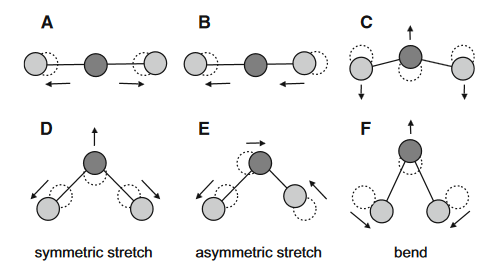
\includegraphics[width = 1 \textwidth]{\currfiledir/Normalmoden.png}
%    \caption{Normal modes of a linear (A-C) and non-linear (D-F) triatomic molecule. The dashed and filled circles represent positions of the atoms at two extremes of motion; arrows show motion in a direction between these extremes. Bending and symmetric stretching preserve mirror symmetry, while asymmetric stretching destroys the symmetries. A linear triatomic molecule also has an additional strain mode perpendicular to the drawing plane, but has only two rotation modes, whereas a non-linear molecule has three. Both also have a single translation mode}
%    \label{fig_Normalmodes}
%\end{figure}
%
%
%%
%\section{Excitation of vibration modes\protect\footnote{Parson, ch. 6.2}} 
%
%Which vibration modes interact with light? The
%They know the results from the 5th semester. The derivation is
%more beautiful here.
%
%Analogous to the transitions between electronic energy levels, a transition dipole can also be used for transitions between the vibration levels with the wave functions $\chi_{m}$ and $\chi_{n}$.
%\begin{equation}
%    \vec{\mu}_{mn} = \Braket{ \chi_{m} | \vec{\mu} | \chi_{n}}
%\end{equation}
%can be defined. For simplification, a two-atomic molecule is assumed, which has only one oscillation normal coordinate $x$. The dipole moment $\vec{\mu}$ can then be developed around the rest position $x = 0$:
%\begin{equation}
%    \vec{\mu}(x) = \vec{\mu}(0) + \frac{\partial \vec{\mu}} {\partial x}\Bigr|_{x=0} x + \dots
%\end{equation}
%For the transitional dipole, the following then applies
%\begin{equation}
%    \vec{\mu}_{mn} = \vec{\mu}(0) \Braket{\chi_{m} | \chi_{n}} + \frac{\partial \vec{\mu}}{\partial x} \Bigr|_{x=0} \Braket{\chi_{m} | x | \chi_{n}} + \dots .
%\end{equation}
%The first summand is zero because the wave functions of the vibration levels are orthogonal. So that the transition dipole does not disappear, must therefore apply:
%\begin{enumerate}
%    \item $\frac{\partial \vec{\mu}}{\partial x}\Bigr|_{x=0} \neq 0$. A transition between the vibration levels in \ch{O2} is therefore forbidden, for example, because the dipole moment disappears due to symmetry.
%    \item $\Braket{ \chi_{m} | x | \chi_{n} }\neq 0$. This is the case with the harmonic oscillator when $m - n = \pm 1$. Thus only transitions between adjacent oscillation levels are allowed.
%\end{enumerate}
%Due to the non-linearity of the potential, transitions $m - n = \pm 2, \pm 3, \dots$ generally also have a non-vanishing transition dipole, but the magnitude of this dipole decreases with increasing order. For molecules with more than two atoms, the Taylor evolution performed above must be extended to several dimensions, corresponding to the normal coordinates.



\printbibliography[segment=\therefsegment,heading=subbibliography]
